\subsection{Комплексная плоскость, сфера Римана и стереографическая проекция. Определения экспоненты $e^z$ и тригонометрических функций $\sin z$, $\cos z$. Определения многозначных функций $\sqrt[n]{z}$, $\operatorname{Ln} z$.}

\subsubsection{Комплексная плоскость.}
 
 Формально вводим символ $i$, такой что $i^2 = -1$.
 
 \begin{definition*} Линейная комбинация обычной единицы и мнимой единицы с вещественными коэффициентами называется \textit{комплексном числом} $z = x + iy$, $x, y \in \mathbb{R}$.  
 	
 Действительная часть числа $z:\ \operatorname{Re} z = x$, мнимая часть числа $z:\ \operatorname{Im} z = y$.
 \end{definition*}
 
 \begin{definition*}
 Каждому комплексному числу $z$ ставится в соответствии \textit{сопряженное}  $\overline{z} = x - iy$.
\end{definition*}
 Можно еще задать комплексное число геометрически:
 
 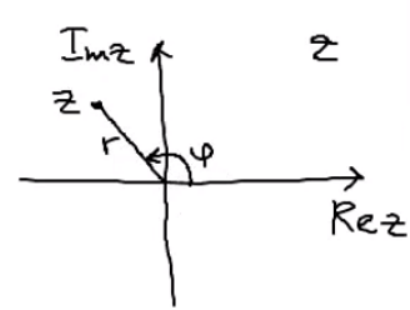
\includegraphics[scale=0.5]{img/1.png}
 
 \begin{definition*}
 Тогда \textit{модуль} числа $z$ -- $r = |z| = \sqrt{z \cdot \overline{z}} = \sqrt{x^2 + y^2}$.
  \textit{Аргумент} числа $z$ -- угол $\varphi$, такой что $x = |z| \cos \varphi,\ y = |z| \sin \varphi$. \end{definition*}
  
  На этом моменте впервые встает вопрос о многозначности  функций.
  
  \begin{definition*}
  Если мы хотим говорить про однозначно выбираемый аргумент, то пишут $\varphi = \operatorname{arg} z \in [0; 2\pi)$ или $(-\pi; \pi]$ --\textit{ главное значение} аргумента. При этом,  $\varphi = \operatorname{Arg}z =\operatorname{arg} z + 2\pi k,k \in \mathbb{Z}$ -- \textit{полный (или многозначный)}  аргумент.
  \end{definition*}

  \begin{definition*}
  \textit{Тригонометрическая запись}  комплексного числа: $z = |z| \cdot (\cos \operatorname{Arg}z + i \sin \operatorname{Arg}z)$.
  \end{definition*}

  \begin{definition*}
  \textit{Показательная форма записи}:  комплексного числа: $z = |z| \cdot e^{i\operatorname{Arg}z}$.
  \end{definition*}

  Комлпексную плоскость обычно обозначают $\mathbb{C}$.

\subsubsection{Сфера Римана и стереографическая проекция.}
На рисунке не окружность,  а сфера единичная. 

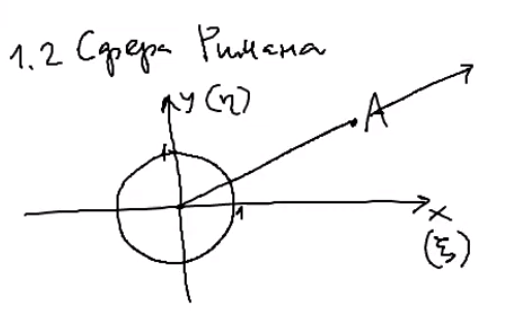
\includegraphics[scale=0.7]{img/2.png}

Рассматриваем вертикальное сечение в плоскости, содержащей ось $\zeta$ и прямую, проходящую через начало координат и точку $A$. Наша сфера выглядит следующим образом (рисунок справа):


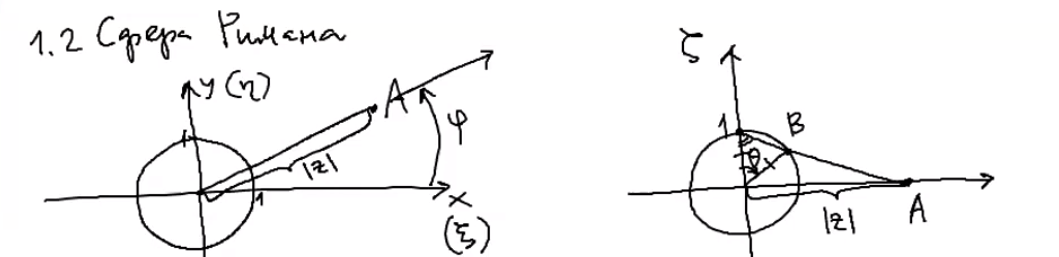
\includegraphics[scale=0.7]{img/3.png}
 
 \begin{definition*}
Отображение $B \longmapsto A$ -- \textit{стереографическая проекция.} Но для нас будет более важным обратное отображение. 
 \end{definition*}

Заметим, что $|z| = \tg \dfrac{\pi - \theta}{2} $ и $\varphi = \operatorname{arg} z$.

 Отсюда несложно вывести (по словам Маевского Е.В.), что $\xi = \dfrac{2x}{1 + |z|^2}, \eta = \dfrac{2y}{1 + |z|^2}, \zeta = \dfrac{|z|^2 - 1}{1 + |z|^2}$.  
 
 Обратные формулы: $x = \dfrac{\xi}{1 - \zeta}$ и $y = \dfrac{\eta}{1 - \zeta}$.
 \\
 \\
В действительном матанализе мы фактически имели две бесконечности (для нас было важно направление): $+\infty $ и $-\infty $. В комплексном матанализе чаще всего не имеет значения, в каком направлении мы идем в бесконечность. Поэтому рассматривается просто \textit{бесконечно удаленная точка }и обозначается $z \to \infty$. Это означает, что $|x|, |y| \to \infty$.  
\\
\\
Можно заметить, что если мы захотим добавить бесконечно удаленную точку к комплексной плоскости, то ей будет соответствовать северный полюс на сфере Римана.  Если мы добавим к комплексной плоскости бесконечно удаленную точку, то  это называется \textit{замкнутой комплексной плоскостью}: $\overline{\mathbb{C}}= \mathbb{C} \cup \{ \infty \}$.  И вот как раз замкнутую комплексную плоскость очень удобно представлять, как сферу Римана.
\\
\\
Стало непонятно, надо ли техать про  сходимость последовательности, поэтому ссылка с таймкодом на лекцию: \href{https://youtu.be/lUqrd4aP3Zc?t=1777}{тык}.
  
  
\subsubsection{Функция комплексной переменной.}
\begin{definition*}
\textit{Функция комплексной переменной }$w = f(z)$ -- отображение, заданное на одной комплексной плоскости и принимающее значения на другой комплексной плоскости. 
\end{definition*}
Считаем, что $w = u + iv$, тогда становится понятно, что $f(z) = u(z) + iv(z)$, где $u(z), v(z) $ -- вещественные функции от комплексной переменной. Еще можно представлять функцию от $z$ как функцию от двух переменных: $f(z) = \widetilde{f}(x, y)$.  Тогда $\widetilde{f}(x, y) = \widetilde{u}(x, y) + i \widetilde{v}(x, y)$.

 Замена переменной:
 \begin{align*}
 \begin{cases}
 	z = x + iy \\
 	\overline{z} = x - iy
 \end{cases} \iff 
 \begin{cases}
 x = \dfrac{z + \overline{z}}{2} \\
 y = \dfrac{z - \overline{z}}{2i}
 \end{cases} 
 \end{align*}
 Тогда $f(z) = \widetilde{f}\left(\dfrac{z + \overline{z}}{2}, \dfrac{z - \overline{z}}{2i}\right)$.
 
 \subsubsection{Определения экспоненты $e^z$ и тригонометрических функций $\sin z$, $\cos z$.}
 
 \begin{definition*}  \textit{Экспонента} $e^z$ в комплексном случае задается двумя  эквивалентными способами:
 	
 	\qquad	1) $e^z := \lim\limits_{n \to \infty} \left(1 + \dfrac zn\right)^n\ \forall z$
 	
 	\qquad	2) $e^z := \sum_{n = 0}^{\infty} \dfrac{z^n}{n!}$
 		
 	На основе этого определения доказываются все те же известные нам алгебраические свойства экспоненты для комплексного случая. 
 \end{definition*}

Тогда можем написать, что $w = e^{x + iy} = e^x \cdot e^{iy} = e^x(\cos y + i\sin y) \implies u  = e^x\cos y,\ v = e^x\sin y$.

\begin{definition*} Косинус в комплексном случае тоже задается двумя эквивалентными способами:
	
	\qquad	1) $\cos z := \dfrac{e^{iz} + e^{-iz}}{2}$ \\
	
	\qquad 2) $\cos z := \sum_{n = 0}^{\infty} \dfrac{(-1)^n z^{2n}}{(2n)!}$
	
	С помощью этих формул можно получить следующее: $$
	\cos z = \dfrac{e^{-y}(\cos x + i\sin x) + e^{y}(\cos x - i\sin x)}{2} = \cos x \ch y - i \sin x \sh y \implies  u =  \cos x \ch y, v = -\sin x \sh y $$
\end{definition*} 


\begin{definition*} Синус в комплексном случае тоже задается двумя эквивалентными способами:
	
	\qquad	1) $\sin z := \dfrac{e^{iz} - e^{-iz}}{2i}$ \\
	
	\qquad 2) $\cos z := \sum_{n = 1}^{\infty} \dfrac{(-1)^{n - 1} z^{2n - 1}}{(2n - 1)!}$
	
	С помощью этих формул можно получить следующее: $$
	\sin z =  \dfrac{e^{-y}(\cos x + i\sin x) - e^{y}(\cos x - i\sin x)}{2i} = \sin x \ch y + i \cos x \sh y \implies  u =  \sin x \ch y, v = \cos x \sh y$$
\end{definition*} 


\subsubsection{Определения многозначных функций $\sqrt[n]{z}$, $\operatorname{Ln} z$.}

\begin{definition*}
	\textit{Комплексным корнем n--ой степени } $\sqrt[n] z, \,z \neq 0$  называется каждое число $w: w^n = z$, где $ n = 2, 3, 4, \dots$
\end{definition*}


\begin{definition*}
	\textit{Полным натуральным логарифмом } $\operatorname{Ln} z$, $ \,z \neq 0$  называется каждое число $w: e^w = z$.
	Составим $z = |z| \cdot e^{i\operatorname{Arg} z} \implies \operatorname{Ln} z  = \ln |z| + i \operatorname{Arg} z = \ln |z| + i \operatorname{arg} z + i 2\pi k, k \in \mathbb{Z}$. Это пример бесконечнозначной функции.
\end{definition*}